The main goal of the thesis is the creation a tool that combines the algorithm estimates for LWE and SIS that we introduced above and can be configured without much knowledge of the workings of the underlying algorithms. To our knowledge there has not been a tool that includes the function of generically searching for secure parameters for both LWE and SIS instances as well as for ring and module variants. Some schemes (e.g. commitment schemes, see \cref{sec:two-problem-search}) depend on the statistical security of either LWE or SIS. We hence include classes respectively to find parameters satisfying this criteria. % TODO: maybe not here just in the section. 
Furthermore, we provide a set of utility classes and methods for most commonly used distributions and norms.
A configuration class allows for a substantial customization of the estimation process.
The tool can either estimate the bit security level of fixed parameter sets or generically search for parameter sets that satisfy a certain bit security level.

% class for distributions... from section this modelling, problems, generic search... Überblick, wie verwendbar,
% automatische norm umwandlung,
% sonstige features
\section{Supported Distributions} \label{sec:supported-distributions}% TODO
The secret distribution used in encryption schemes based on LWE or SIS can either distributed according to a Gaussian or a uniform distribution. The error distribution in LWE must be a Gaussian distribution with parameter $\alpha$. In general, if both error and secret are sampled in LWE are sampled according to Gaussian distributions their parameters may differ. Currently, however, the \textit{estimator} only supports secrets that follow a uniform distributions or a Gaussian distribution with the same paramter as the error distribution.

\subsection{Gaussian Distribution}
In some applications we receive a Gaussian distribution as input but require a bound in some norm in order to estimate the hardness of an SIS instance. Hence, we need to transform a Gaussian with parameter $s  = \sqrt{2 \pi} \sigma$ into a bound $\beta$ given some security parameter $\texttt{sec}$. Note that a $n$-dimensional Gaussian $D_{\mathbf{Z}^n, s}$ can be sampled by combining samples from $n$ independent one-dimensional Gaussians $D_{\mathbf{Z}, s}$ \cite{GJS15}. %TODO check

For a Gaussian distribution and a random variable $X$ with $X \sim D_{\mathbf{Z}, s}$, the following holds: % put as theorem, also for norm inequalities

\begin{equation}
    \text{Pr}\left[ |X| \geq \beta \right] \leq 2 e^{-\pi \|\mathbf{v}\|^2/s^2}
\end{equation}

We demand $2 e^{-\pi \beta^2/s^2} \approx 2^{-\texttt{sec}}$ with $\beta = \|\mathbf{v}\|$  and obtain

\begin{align*}
    2 e^{-\pi \beta^2/s^2}   & \approx 2^{-\texttt{sec}}                               \\
    -\pi \frac{\beta^2}{s^2} & \approx (-\texttt{sec} - 1)\ln (2)                      \\
    \beta                    & \approx s \sqrt{\frac{(\texttt{sec} + 1) \ln(2)}{\pi}}.
\end{align*}

\begin{theorem}[Gaussian to Bound]
    Given a Gaussian distribution $D_{\mathbf{Z}^n, s}$ with width parameter $s  = \sqrt{2 \pi} \sigma$ and a security parameter $\texttt{sec}$, we can compute a bound $\beta$ such that a sample $\mathbf{v}$ drawn from $D_{\mathbf{Z}^n, s}$ satisfies $\text{Pr}\left[ \|\mathbf{v}\| \geq \beta \right] \leq 2^{-\texttt{sec}}$ as follows:
    \begin{equation}
        \beta  \approx s \sqrt{\frac{(\texttt{sec} + 1) \ln(2)}{\pi}}.
    \end{equation}
\end{theorem}

The resulting bound $\beta$ is an $\ell_2$-norm bound. % TODO: distributions is changes => thanks Marc! (also noticed that it doesn't make sense to have componentwise and L2)

We provide the classes $\texttt{GaussianAlpha}$, $\texttt{GaussianSigma}$ and $\texttt{GaussianS}$ to allow for the most flexibility in specifying a Gaussian distribution.

\subsection{Uniform Distribution}
For uniform distributions, we support all distributions that are supported by the \textit{estimator}, namely, uniform $\mod q$, uniform in the interval $[a,\dots,b]$ and a sparse uniform distribution with parameters $((a,b), h)$, where exactly $h$ components are in the interval $[a,\dots,b] \setminus \{0\}$ and all other components are zero. Note that we only consider discrete distributions are over $\mathbb{Z}$.

We can estimate the corresponding standard deviation for a Gaussian distribution by computing the variance of the uniform distribution. Given an lower and upper bound $(a, b)$, the variance for a discrete uniform distribution is defined as $\sigma^2 = \frac{(b - a + 1)^2 - 1}{12}$. For a uniform distirbution $\mod q$ we set $a = -\left\lfloor \frac{q}{2} \right\rfloor, b = \left\lfloor \frac{q}{2} \right\rfloor$.

For a sparse discrete $n$-dimensional uniform distirbution $\mathcal{U}_h$ with an additional sparseness parameter $h$ and a random variabel $X \sim \mathcal{U}_h$, we can compute the expected values $\mathbb{E}(X^2)$ and $\mathbb{E}(X)^2$ as follows \cite{APS15}:
% TODO maybe figure out why that is so

\begin{align}
    \mathbb{E}(X^2) & = \frac{h}{n} \cdot \frac{2b^3 + 3b^2 + b - 2a^3 + 3a^2 - a}{6(b - a)} \\
    \mathbb{E}(X)^2 & = \frac{h}{n} \cdot \frac{b (b + 1) - a(a - 1)}{2(b - a)}
\end{align}

and obtain the variance $\text{Var}(X) = \mathbb{E}(X^2) - \mathbb{E}(X)^2$.



\section{Norms bound estimates} \label{sec:norm-bounds}% TODO: check
%TODO: write some prose about why we need that
% TODO: make sure that it is clear that these are bounds!!!
In practical scenarios, oftentimes we require that the bound of a result does not exceed a certain value to guarantee correctness. In addition, we have seen that estimation algorithms rely on bounds in different $\ell_p$-norms. For example, the combinatorial attack in \cref{sec:combinatorial} needs a bound in $\ell_\infty$ norm, whereas the dual attack in \cref{sec:dual-attack} uses bounds in the Euclidean norm. We thus need a way to bound a value of a bound in one norm by a value in a different norm. In our tool, we define a norm class with parameter $p$ and provide a  method $\texttt{to\_lp()}$ for conversions into all other norms mentioned here. Recall the norm definitions in \cref{sec:norms}.

It is easy to see that for any $\infty \geq p \geq q \geq 1$ the following two inequations hold
\begin{align}
    \| f \|_p & \leq \| f \|_q \label{eq:norm-inf-leq-1}.
\end{align} % maybe replace norm4 with this one % maybe replace norm4 with this one
In addition, if we apply Hölder's inequality to finite vector spaces as in \cite{norm-relations} we obtain the following Lemma:
\begin{lemma}
    For $1 \leq p \leq q \leq \infty$ it holds that
    \begin{align}
        \lim_{q' \rightarrow q}\| f \|_p & \leq n^{\frac{1}{p} - \frac{1}{q'}}\| f \|_q' \label{eq:norm-1-leq-inf}
    \end{align} % TODO: show full proof https://math.stackexchange.com/questions/218046/relations-between-p-norms
\end{lemma}


% \begin{proof}
%     Folowing \cite{norm-relations}, we apply Hölder's inequality on $n$ dimensional vector spaces. For $\mathbf{x}, \mathbf{y} \in \mathbb{R}^n$ Hölder's inequality states that
%     \begin{align*}
%         \sum_{i=1}^n |x_i| |y_i| \leq \left(\sum_{i=1}^n |a_i|^s\right)^{\frac{1}{s}}.
%     \end{align*}
% \end{proof}

% \begin{align}
%     \| f \|_1      & \leq \sqrt{n} \| f \|_2 \label{norm1}                                                                         \\
%     \| f \|_1      & \leq n \| f \|_\infty \label{norm2}                                                                           \\
%     \| f \|_2      & \leq \sqrt{n} \| f \|_\infty \;\;(\text{because of }  \sqrt{n} \| f \|_2 \leq n \| f \|_\infty) \label{norm3} \\
%     \| f \|_\infty & \leq \| f \|_1 \label{norm4}
% \end{align}

Let $\mathcal{O}_K$ be the ring of integers of a number field $K=\mathbb{Q}(\theta)$, where $\theta$ is an algebraic number and $\sigma$ denote the canonical embedding as defined in \cite{DPSZ12}. Then, according to \cite[Theorem~7]{DPSZ12} for $f \in \mathcal{O}_K$  the following inequations hold: % TODO: why?
\begin{align}
    \| f \|_\infty         & \leq \| \sigma(f) \|_\infty \label{norm5}, \\
    \| \sigma(f) \|_\infty & \leq \| f \|_1 \label{norm6}.
\end{align}
(We assume that the constant $C_m$ used in the original Theorem is $1$ for $m$ a power of $2$ \cite[Lemma~3]{DPSZ12}.) From the above inequations, we obtain the following theorems that we use in the method $\texttt{to\_lp()}$.
\begin{theorem}[Relationships Between Norm Bounds \cite{BDLOP18,DPSZ12}]\label{th:norm-rel}
    Given a ring element $f \in \mathcal{O}_K$ as defined above, then we can bound norms by $\ell_p$-norms as follows:
    \begin{itemize}
        \item From \cref{eq:norm-1-leq-inf}, it follows that
              \begin{equation}\label{eq:l1-to-p}
                  \begin{aligned}
                      \| f \|_1 & \leq n^{1 - \frac{1}{2}} \| f \|_2 = \sqrt{n} \| f \|_2, \\
                      \| f \|_1 & \leq n^{1 - \frac{1}{p}} \| f \|_p,                      \\
                      \| f \|_1 & \leq n^{1 - 0} \| f \|_\infty = n \| f \|_\infty.
                  \end{aligned}
              \end{equation}
        \item From \cref{eq:norm-inf-leq-1}, it follows that
              \begin{align}
                  \| f \|_2 & \leq \sqrt{n}  \| f \|_1.
              \end{align}
              From \cref{eq:norm-1-leq-inf} and with $2\leq p < \infty$, we get that
              \begin{equation}\label{norm2}
                  \begin{aligned}
                      \| f \|_2 & \leq n^{\frac{1}{2} - \frac{1}{p}} \| f \|_p,                      \\
                      \| f \|_2 & \leq n^{\frac{1}{2} - 0} \| f \|_\infty =\sqrt{n}  \| f \|_\infty.
                  \end{aligned}
              \end{equation}
        \item From \cref{eq:norm-1-leq-inf,eq:norm-inf-leq-1} and with $p\geq 2$, it holds that
              \begin{equation}\label{norm1}
                  \begin{aligned}
                      \| f \|_p & \leq  \| f \|_1,               \\
                      \| f \|_p & \leq  \| f \|_2,               \\
                      \| f \|_p & \leq \sqrt{n}  \| f \|_\infty.
                  \end{aligned}
              \end{equation}
        \item From \cref{eq:norm-inf-leq-1}, it follows that
              \begin{align*}
                  \| f \|_\infty & \leq  \| f \|_1, \\
                  \| f \|_\infty & \leq  \| f \|_2, \\
                  \| f \|_\infty & \leq \| f \|_p.
              \end{align*}
        \item From \cref{norm6,eq:l1-to-p} it follows that
              \begin{align*}
                  \| \sigma(f) \|_\infty \leq \| f \|_1,                     \\
                  \| \sigma(f) \|_\infty \leq \sqrt{n} \| f \|_2,            \\
                  \| \sigma(f) \|_\infty \leq n^{1 - \frac{1}{p}} \| f \|_p, \\
                  \| \sigma(f) \|_\infty \leq n \| f \|_\infty.
              \end{align*}
    \end{itemize}
    Likewise, we get the following bounds for the $\ell_\infty$-norm on the canonical embedding which we call $\mathcal{C}_\infty$:
    \begin{itemize}
        \item From \cref{eq:l1-to-p,norm5}, it follows that $\| f \|_1 \leq  n \| \sigma(f) \|_\infty$.
        \item From \cref{norm2,norm5}, it follows that $\| f \|_2 \leq  \sqrt{n} \| \sigma(f) \|_\infty$.
        \item From \cref{norm1,norm5}, it follows that $\| f \|_p \leq  \sqrt{n} \| \sigma(f) \|_\infty$ for $2 < p < \infty$.
        \item From \cref{norm5}, it follows that $\| f \|_\infty \leq  \| \sigma(f) \|_\infty$.
    \end{itemize}
\end{theorem}

We also want to be able to add and multiply bounds from different norms. Note that the degree of the polynomial of the underlying ring to which we apply the norms must match. To add two bounds we simply bound the second addend by the used norm of the first as described in \cref{th:norm-rel} and add both bounds to obtain a bound in the norm of the first addend. It is slightly more complicated for multiplication and we state the results in the next theorem.

\begin{theorem}[Multiplication of Norm Bounds \cite{BDLOP18, DPSZ12}]
    Let $f$ be defined as above and let $g \in \mathcal{R}_q$ where $g = \sum_i \overline{g}_i X^i$ where $g_i \in \left[-(q-1)/2, (q-1)/2\right]$ and $\overline{g}_i = g_i \mod q$ as in \cite{BDLOP18}. We then can define the following inequations for multiplication according to \cite{BDLOP18}:

    \begin{itemize}
        \item If $\|f\|_\infty \leq \beta, \|g\|_1 \leq \gamma$ then $\|f \cdot g\|_\infty \leq \beta \cdot \gamma$.
        \item If $\|f\|_2 \leq \beta, \|g\|_2 \leq \gamma$ then $\|f \cdot g\|_\infty \leq \beta \cdot \gamma$.
    \end{itemize}

    Let $x, y \in \mathcal{O}_K$. (Again, we assume that $C_m = 1$ in the original theorem.) Then, the following inequation holds according to \cite{DPSZ12}:
    \begin{align*}
        \| x \cdot y \|_\infty         & \leq n^2 \cdot \| x \|_\infty \cdot \| y \|_\infty         \\
        \| \sigma(x \cdot y) \|_\infty & \leq  \| \sigma(x) \|_\infty \cdot \| \sigma(y) \|_\infty.
    \end{align*}
\end{theorem}




\section{Problem Classes}
We now present the problem classes in $\texttt{lattice\_parameter\_estimation/problem}$ (see \cref{fig:problem-classes}).

\begin{figure}[h]
    \centering
    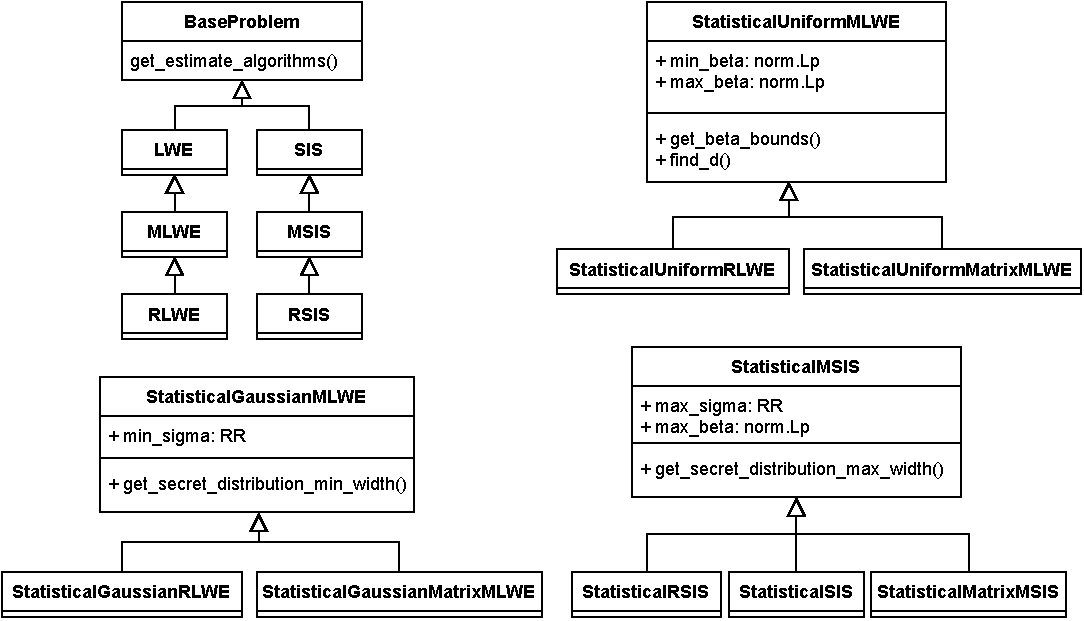
\includegraphics[width=1\textwidth]{graphics/problem_classes.pdf}
    \caption{Problem classes}\label{fig:problem-classes}
\end{figure}

$\texttt{LWE}$ and $\texttt{SIS}$ inherit from the base class $\texttt{BaseProblem}$ respectively. All instances provide a method $\texttt{get\_estimate\_algorithms()}$ that returns a list of algorithm instances that can be executed by the function $\texttt{estimate()}$. Furthermore, any instance of $\texttt{BaseProblem}$ can be compared to a bit security level (for more details, we refer the reader to the documentation). The $\texttt{LWE}$ class is initialized by the secret dimension $n$, a modulus $q$, the number of samples $m$, a $\texttt{secret\_distribution}$ and a $\texttt{error\_distribution}$. Both $\texttt{secret\_distribution}$ and $\texttt{error\_distribution}$ must be instances of the class $\texttt{distributions.Distribution}$. Instead of $\texttt{secret\_distribution}$ and $\texttt{error\_distribution}$, a bound of type $\texttt{norm.BaseNorm}$ must be set for $\texttt{SIS}$. Note that both {distributions.Uniform} and {distributions.Gaussian} are instances of $\texttt{norm.BaseNorm}$ and can thus be used as a bound. We compute the bound for a given distribution instance as described in \cref{sec:supported-distributions}.

For ring and module variants $\texttt{RLWE}$, $\texttt{RSIS}$ and $\texttt{MLWE}$, $\texttt{MSIS}$ respectively $n$ denotes the degree of the polynomial of the underlying ring $\mathcal{R}_q$. The module variants $\texttt{MLWE}$ and $\texttt{MSIS}$ take an addition parameter $d$ for the rank of the module.

While there exist special cases where the ring structure of problem instances can be exploited in an attack on LWE or SIS, % TODO: find examples
in general, the hardness of ring and Module variants is estimated by interpreting the coefficients of elements of $\mathcal{R}_q$ as vectors in $\mathbb{Z}_q^n$ \cite{ACDDPPVW18}. If we take into account the considerations we presented in \cref{sec:ring-module}, we can thus reduce ring and Module instances as follows when calling $\texttt{get\_estimate\_algorithms()}$ on the ring and module variant of $\texttt{LWE}$ and $\texttt{SIS}$:
\begin{itemize}
    \item RLWE$_{n, q, m, \chi} \longrightarrow$ LWE$_{n, q, m \cdot n, \chi}$
    \item MLWE$_{n, d, q, m, \chi} \longrightarrow$ LWE$_{n \cdot d, q, m \cdot n, \chi}$
    \item RSIS$_{n, q, m, \beta} \longrightarrow$ SIS$_{n, q, m \cdot n, \beta}$
    \item MSIS$_{n, d, q, m, \beta} \longrightarrow$ SIS$_{n \cdot d, q, m \cdot n, \beta}$
\end{itemize}


In addition to the base problem variants, we define some statistically secure variants for both LWE and SIS since some schemes depend on the unconditional hardness of either LWE or SIS. More precicely, we ask for parameters such an arbitrary powerful attacker can only break the scheme with probability less than $2^{-\texttt{sec}}$.

\paragraph{$\texttt{StatisticalGaussianMLWE}$.} For LWE, we define a statistically secure variant over a Gaussian distribution and over a uniform distribution. $\texttt{StatisticalGaussianMLWE}$ follows Corollary 7.5 and Theorem 7.4 in \cite{LPR13}. The mapping of the parameters in \cite{LPR13} to the usage in this work can be found in \cref{tab:mapping-LPR13}. We obtain the following theorem:

\begin{theorem}[Statistically Secure MLWE Over a Gaussian Distribution \cite{LPR13}]
    Let $\mathcal{R}$ be the ring of integers in the $m'$th cyclotomic number field $K$ of degree $n$, and $q \geq 2$ an integer.
    For positive integers $m \leq m + d \leq \text{poly}(n)$, let $\mathbf{A} = [ \mathbf{I}_{[m]} \mid \bar{\mathbf{A}}] \in (\mathcal{R}_q)^{[m] \times [m+d]}$, where $\mathbf{I}_{[m]} \in (\mathcal{R}_q)^{[m] \times [m]}$ is the identity matrix and $\bar{\mathbf{A}} \in (\mathcal{R}_q)^{[m] \times [d]}$ is uniformly random.
    Then with probability $1 - 2^{-\Omega(n)}$ over the choice of $\bar{\mathbf{A}}$, the distribution of $\mathbf{A}\mathbf{x} \in (\mathcal{R}_q)^{[m]}$ where each coordinate of $\mathbf{x} \in (\mathcal{R}_q)^{[m+d]}$ is chosen from a discrete Gaussian distribution of parameter $s > 2n \cdot q^{m / (m+d) + 2/(n (m+d))}$ over $\mathcal{R}$, satisfies that the probability of each of the $q^{n m}$ possible outcomes is in the interval $(1 \pm 2^{-\Omega(n)}) q^{-n }$ (and in particular is within statistical distance $2^{-\Omega(n)}$ of the uniform distribution over $(\mathcal{R}_q)^{[m]}$). % TODO change [x]times[y] notation???
\end{theorem}
% TODO: anything more? can you provide an intuition?

If a security parameter is passed and $\texttt{sec} > n$, we raise an exepction.
The resulting minimal standard deviation is stored in the instance variable $\texttt{min\_sigma}$ and the corresponding distribution can be obtained by calling $\texttt{get\_secret\_distribution\_min\_width()}$ on the class instance.



\paragraph{$\texttt{StatisticalUniformMLWE}$.} The authors of \cite{BDLOP18} describe statistically secure MLWE instances over a Uniform distribution with invertible elements. The samples $(\mathbf{A}', h_{\mathbf{A}'}(y))$ of the resulting MLWE instance are within statistical distance $2^{-\texttt{sec}}$ of $(\mathbf{A}', \mathbf{u})$ for uniformly distributed $\mathbf{u}$. % TODO: check formulation

We obtain the following theorem (for a mapping of the parameters, see \cref{tab:mapping-BDLOP18}): %TODO 

\begin{theorem}[Statistically Secure MLWE Over a Uniform Distribution \cite{BDLOP18}]
    Let $1 < d_2 < n$ be a power of 2. If $q$ is a prime congruent to $2d_2 + 1 \;(\text{mod } 4d_2)$ and
    \begin{equation}
        q^{m/(m+d)} \cdot 2^{2 \texttt{sec}/((m+d)\cdot n)} \leq 2 \beta < \frac{1}{\sqrt{d_2}} \cdot q^{1/d_2}
    \end{equation}
    then any (all-powerful) algorithm $\mathcal{A}$ has advantage at most $2^{-\texttt{sec}}$ in solving $\text{DKS}_{m,m+d,\beta}^\infty$, where $\text{DKS}^\infty$ is the decisional knapsack problem in $\ell_\infty$-norm.
\end{theorem}


Hence, we have:
\begin{align}
    \beta_{min} & = \frac{q^{m/(m+d)} \cdot 2^{2 \texttt{sec}/((m+d)\cdot n)}}{2} \\
    \beta_{max} & = \frac{1}{2\sqrt{d_2}} \cdot q^{1/d_2} - 1
\end{align}
% TODO: explain how to arrive at 2*\texttt{sec} instead of 256, für generellen \texttt{sec} parameter ...
% proof zum Beispiel im Anhang ...

The variable $d_2$ can be passed as an argument. If it is not passed, we try to find $d_2$ by iterating over all powers of $2$ that are smaller than $n$.
The resulting bounds are converted to $\ell_\infty$ and stored in the instance variables $\texttt{min\_beta}$ and $\texttt{max\_beta}$. We also provide an instance method $\texttt{get\_beta\_bounds()}$ to obtain a tuple of both.

For both statistically secure MLWE variants, we include the corresponding ring versions $\texttt{StatisticalGaussianRLWE}$ and $\texttt{StatisticalUniformRLWE}$ for $d=1$ and matrix versions $\texttt{StatisticalGaussianMatrixMLWE}$ and $\texttt{StatisticalUniformMatrixMLWE}$ for which the width and height of the matrix $\mathbf{A}$ in \cite{LPR13} can be passed instead of $m$ and $d$. % TODO: include instead of included?
% TODO: explain why this doesn't work for LWE


\paragraph{$\texttt{StatisticalMSIS}$.} We can find parameters for a statistically secure MSIS instance by following Section 4.1 of \cite{DOTT21}. The mapping of the parameters in \cite{DOTT21} is shown in \cref{tab:mapping-DOTT21}. More specifically, we ask to find a MLWE instance where the probability that non zero elements $\mathbf{r}$ in the Euclidean ball $B_{m}(0, 2B)$ satisfy $\hat{\mathbf{A}}_1 \cdot \mathbf{r} = \mathbf{0}$ is smaller than $2^{-\texttt{sec}}$. % TODO check that this is not a quote

The number of elements in $B_{m+d}(0, 2B)$ can be estimated from above as $|B_{m+d}(0, 2B)| \ll (2 \pi e /((m+d) n))^{(m+d) n/2} \cdot (2 B)^{(m+d) n}$. The scheme is statistically binding if the probability that non zero elements in $B_{m+d}(0, 2B)$ of radius $2B$ in $\mathcal{R}_q^{m+d}$ map to $\mathbf{0}$ in $\mathcal{R}_q^{m}$ is negligible. Hence, it must hold that $|B_{m+d}(0, 2B)|/q^{m n} \leq 2^{-\texttt{sec}}$ and we get:

% TODO: look for bound of ball without o(...) if change also change in docstring, check out wikipedia => heuristic. maybe find version not heuristic?
% add that this is approximation, see https://en.wikipedia.org/wiki/Volume_of_an_n-ball
% for small n?

\begin{align}
    \left(\sqrt{\frac{2 \pi e}{(m+d) \cdot n}} \cdot 2 B\right)^{(m+d) \cdot n} & \leq 2^{-\texttt{sec}} \cdot q^{m\cdot n}                                                                       \\
    B                                                                           & \leq 2^{\frac{-\texttt{sec}}{(m+d)\cdot n} - 1} \cdot q^\frac{m}{m+d} \cdot \sqrt{\frac{(m+d)\cdot n}{2 \pi e}}
\end{align}

We convert the bound $B$ to a Gaussian over $\ell_2$-norm by following the procedure described in \cref{sec:norm-bounds}: % TODO: add appropriate reference

\begin{equation}
    s  \approx x \sqrt{\frac{\pi}{(\texttt{sec} + 1) \ln(2)}}
\end{equation}

% TODO: rephrase to obtain a lemma?
The resulting parameters $B$ and $s$ can be accessed by the instance variables $\texttt{max\_sigma}$ and $\texttt{max\_beta}$ or by calling $\texttt{get\_secret\_distribution\_max\_width()}$ on the class instance.

As for statistically secure MLWE we again include a matrix version $\texttt{StatisticalMatrixMSIS}$ and a ring $\texttt{StatisticalRSIS}$ by setting $d=1$. In addition, the proof also applies to the base SIS variant and hence we include $\texttt{StatisticalSIS}$. Here the height of the matrix $n$ becomes the rank of the modulus in the MSIS instance, i.e. $d=n$, and the degree of the polynomial is $1$.




\section{Parameter Search and Configuration Options}
We now describe the main parameter search and estimate configuration options in our tool. The configuration can be customized by using the class $\texttt{algorithms.Configuration}$ and passed as an optional argument of $\texttt{param\_search.generic\_search()}$. It is also possible to directly estimate the cost of a list of parameter problems by calling the function $\texttt{problem.estimate()}$. For more details we again refer to the documentation.

\paragraph{Cost Models.} Attacks that use BKZ for lattice reduction require a cost model to estimate the number of CPU cycles in the SVP subroutine. Default cost models are shown in \cref{tab:costmodels}. We distinguish between estimates for classical, quantum, sieving and enumeration and each of these categories can be deselected by setting the respective parameter to $\texttt{False}$. At least one of classical and quantum and of sieving and enumeration respectively must be selected to make use of the default cost models.

Note that classical and quantum cost models cannot be directly compared with each other. The number of operations per second that can be executed by a quantum computer may be significantly smaller than for classical computers. % TODO add more?

If all are unselected custom cost models must be specified and passed as an argument. We included an option of taking the most conservative estimate for each category combination for a more efficient parameter search or estimation. Furthermore, we assigned a priority value on an ordinal scale to each cost model which enables us to first run cost models that yield a lower cost and thus terminate the estimation process earlier for an insecure parameter set. The priority values of the default cost models are derived from \cref{fig:costmodels}.
\begin{figure}[h]
    \centering
    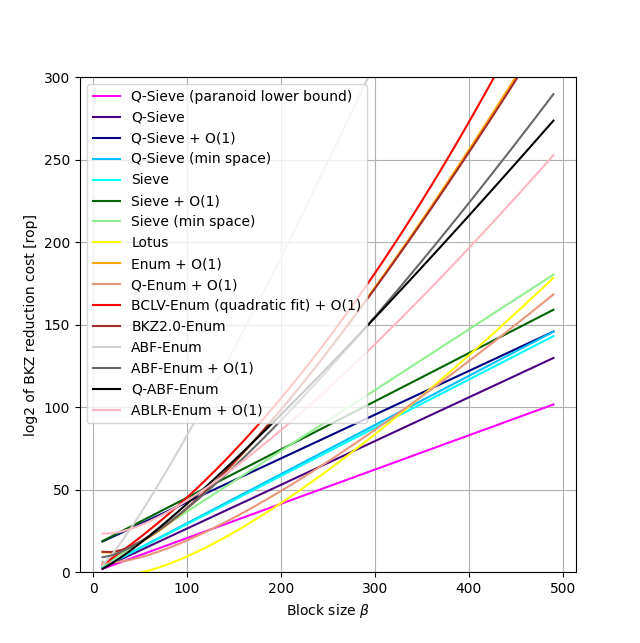
\includegraphics[width=0.7\textwidth]{graphics/cost_models.png}
    \caption{Cost models}\label{fig:costmodels}
\end{figure}
The number of BKZ rounds can be configured by passing a function with parameters $\texttt{beta, d}$ where $\texttt{beta}$ is the block size and $\texttt{d}$ the lattice dimension. In the default configuration we use the more conservative Core-SVP model $\texttt{algorithms.BKZ\_SVP\_repeat\_core}$ \cite{ADPS16} in which the polynomial factor of the runtime complexity of BKZ is completely ignored. In addition, we provide a more realistic model $\texttt{algorithms.BKZ\_SVP\_repeat\_8d}$ for a BKZ cost of $8 \cdot d \cdot t_k$ BKZ rounds where $d$ again referes to the lattice dimension and $t_k$ is the number of clock cycles required for the SVP subroutine (see \cref{sec:bkz-8d}). % TODO maybe add a little more of evaluation here


\subsection{Generic Search and Estimate Algorithms}
The main functionality of our tool is encapsulated in the function $\texttt{param\_search.generic\_search()}$. The high-level idea of the search is presented in \cref{alg:generic-search}. We begin with an initial parameter set. We then create a list of problem instances generated by a $\texttt{parameter\_problem}$ function and estimate the cost of all instances in the list. If the list contains multiple SIS instances or multiple LWE instances, we attempt to reduce the instances to the easiest problem instance respectively. % TODO: include how, \cref{sec:problem-reduction} 
Once the $\texttt{estimate}$ function finds an instance that is insecure (i.e. the estimated attack cost in clock cycles is smaller than $2^{\texttt{sec}}$), it terminates the estimation procedure and returns an insecure result. We then use the $\texttt{next\_parameters}$ function to generate a list L of (multiple) new parameter sets from our current parameter set and sort each of the new parameter sets into an ordered list (duplicates are not accepted). The order is defined by a $\texttt{parameter\_cost}$ function. In the next step we retrieve the parameter set with the lowest cost from L and repeat the procedure until the cost estimation step returns a secure result. The result includes the estimates for all cost models and algorithms.

\begin{algorithm2e} % TODO: check if block is not of dimension kxk
    \SetKwBlock{Begin}{function}{end function}
    \Begin(generic\_search(sec, initial\_params, next\_parameters, parameter\_cost,  problem\_instance)) % TODO nxn???
    {
        L = OrderedList(initial\_params)\\
        \While{L $\neq \emptyset$}{
            current\_params = L.pop() \\
            instances = parameter\_problem(current\_params) \\
            result = estimate(instances, sec) \\
            \If{result is secure}{
                Return result\\
            }
            \Else{
                next\_param\_sets = next\_parameters(current\_params)\\
                \ForAll{param\_set in next\_param\_sets}{
                    sort param\_set into L according to parameter\_cost function\\
                }
            }
        }

    }
    \caption{Generic search} \label{alg:generic-search}
\end{algorithm2e}

The $\texttt{estimate}$ function can be configured to run in parallel in the configuration which may speed up the search, in particular if many cost models need to be tested (e.g. with configuration setting $\texttt{conservative=False}$ and long running algorithms like $\texttt{ARORA\_GB}$, $\texttt{CODED\_BKW}$ and $\texttt{PRIMAL\_DECODE}$ are used. The list of used algorithms can be changed in the configuration. We recommend to include $\texttt{PRIMAL\_USVP}$ for LWE instances and $\texttt{LATTICE\_REDUCTION}$ for SIS instances to make full use of early termination since the estimate algorithms for these attacks have a short runtime and yield relatively low cost estimates.


\cref{fig:SIS-algs}, \ref{fig:LWE-algs-small} and \ref{fig:LWE-algs-large} show the plots of runtime and performance tests for the various algorithms that can be used in our tool. In accordance with the results, we assigned priority values on an ordinal scale to the estimation algorithms. In \cref{tab:lwe-alg-prio} and \ref{tab:sis-alg-prio} we present the list of algorithms and their corresponding priority values and justify our choice. Algorithms with a smaller priority are expected to yield relatively good results quickly and can therefore be executed first. If the estimate result does not satisfy the specified security requirement we can terminate the estimation process early in order to maximize the efficiency of our search. Note that directly comparing the results for different algorithms, while convenient, is not always admissible as the compared algorithms may rely on different assumptions. Some algorithms may compute a more realistic cost while others may return a more conservative or even paranoid cost estimate (e.g. BKZ is used with the Core-SVP paranoid lower bound). The results have to be weighted carefully in order to guarantee the security of a given scheme in the forseable future while trying to keep the cost of using the scheme as low as possible. % TODO maybe move to conclusion...

\begin{figure}[]
    \centering
    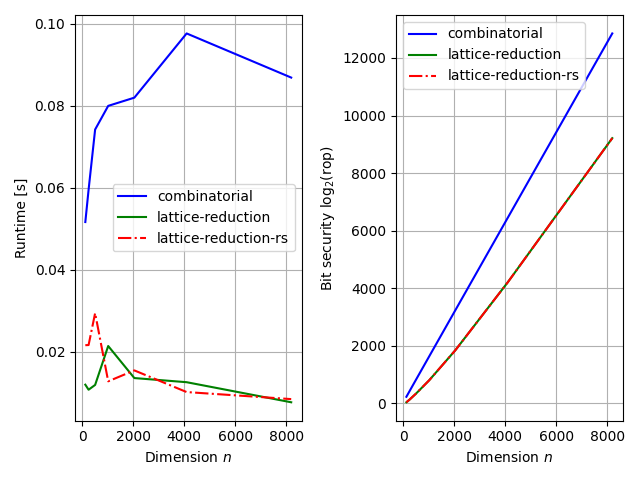
\includegraphics[width=0.8\textwidth]{graphics/SIS_stddev=2,828_plots_1s.png}
    \caption{SIS instance with $\sigma=2.828,\; m=n^2, \; 2^{2n} < q < 2^{2n+1}$}\label{fig:SIS-algs}
\end{figure}

\begin{figure}[]
    \centering
    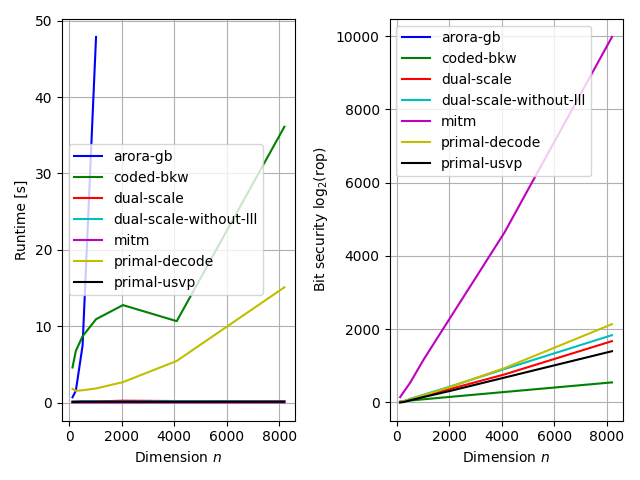
\includegraphics[width=0.8\textwidth]{graphics/LWE_stddev=0,125_plots_200s.png}
    \caption{LWE instance with $\sigma=0.125,\; m=\infty, \; 2^{n} < q < 2^{n+1}$}\label{fig:LWE-algs-small}
\end{figure}

\begin{figure}[]
    \centering
    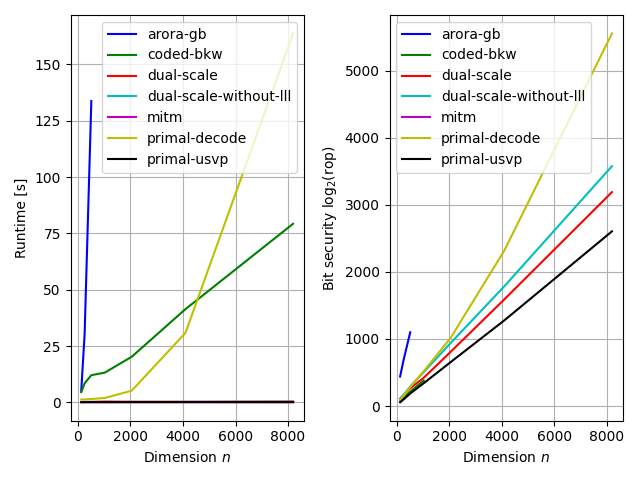
\includegraphics[width=0.8\textwidth]{graphics/LWE_stddev=2,828_plots_200s.png}
    \caption{LWE instance with $\sigma=2.828,\; m=\infty, \; 2^{n} < q < 2^{n+1}$}\label{fig:LWE-algs-large}
\end{figure}

% TODO: how does dual attack without LLL work???
\begin{table}
    \centering
    \begin{tabular}[]{lll}
        \toprule
        Algorithm                 & Priority & Justification                                       \\\hline
        Meet-in-the-Middle        & 5        & fastest, high cost estimate, as prefilter           \\
        Primal-uSVP               & 10       & fast, low cost estimatate estimates                 \\
        Dual Attack               & 20       & fast, often higher estimates than primal-usvp       \\
        Dual Attack (without LLL) & 30       & fast, often higher estimates than dual              \\
        Coded-BKW                 & 90       & slow, somtimes very low cost estimate               \\
                                  &          & (for small stddev), does not always yield results   \\
        Decoding Attack           & 100      & slow, often higher estimates than faster algorithms \\
        Arora-Ge                  & 200      & extremely slow, often higher estimates,             \\
                                  &          & does not always yield results                       \\
        \bottomrule
    \end{tabular}
    \caption{LWE estimate algorithm priorities}\label{tab:lwe-alg-prio}
    \vspace{1cm}
    \begin{tabular}[]{lll}
        \toprule
        Algorithm                     & Priority & Justification                            \\\hline
        Lattice Reduction \cite{MR09} & 5        & fastest, low cost estimates              \\
        Lattice Reduction \cite{RS10} & 7        & same results as lattice-reduction,       \\
                                      &          & not always applicable                    \\
        Combinatorial Attack          & 10       & fast, often slightly higher cost results \\
        \bottomrule
    \end{tabular}
    \caption{SIS estimate algorithm prioritie}\label{tab:sis-alg-prio}
\end{table}

% TODO first finish section on algorithms
% - include plots
% - write about pro/cons
% - maybe add section of cost comparison for the algorithms of the previous section
